\section{Our implementation}
\label{sec:our_implementation}

\subsection{Short summary of the functionality of our simulator}

Using the Fourier method, we created a Python application simulating the time development of the quantum mechanical wave function.
We use ray tracing to visualize the resulting volumetric probability density.
The visualization requires the sampling of a 3D data set on a discretized grid.
This makes it impossible to fully reconstruct the wave function that we simulated using only a finite resolution to begin with.
In order to fight sampling artifacts, we deploy a state-of-the-art triquadratic reconstruction filter recently proposed by Balázs Csébfalvi \cite{csebfalvi2023}.

\subsection{Technologies in use}

We choose Python \cite{van1995python} as our programming language because there is a vast amount of helpful tools implemented to use with it that specifically aim towards leveraging the difficulty of writing mathematical and physics-related simulations.
The majority of these tools are written in hardware-friendly languages such as Fortran, C, or C++.
However, they come with an easy-to-use \acrfull{api} that can be accessed from high-level programming languages.
In these modern languages, such as Python, one works on a higher abstraction level, usually not dealing with memory management or pointer arithmetic.
Out implementation heavily depends on the Numpy library \cite{harris2020array}.
NumPy is a library that can be utilized to work efficiently with large arrays and tensors performing computationally intensive operations.
A similar library is SciPy \cite{2020SciPy-NMeth}, also used in our program.
For 3D visualization, we choose to use VisPy \cite{vispy}.
This library provides an excellent basic set of features to handle virtual cameras and create scenes but also enables us to go deeper and write our own \acrshort{gpu} shader code.
We made use of this to modify the default volume visualization code to fit our needs.

\subsection{GPU parallelization and Just In Time compilation}

The Fourier method described in section \ref{sec:used_method} opens up the possibility to implement the simulation on the \acrshort{gpu}.
Using \acrshort{gpu} acceleration is one of our contributions to the already existing implementation used by Géza István Márk and Péter Vancsó.
The \acrfull{cuda} toolkit is often used for parallel computational tasks implemented on the \acrshort{gpu} \cite{cuda2008}.
It comes with a powerful \acrshort{gpu} based \acrshort{fft} implementation.
To use \acrshort{cuda} with Python, we selected the CuPy wrapping library \cite{cupy_learningsys2017} that provides abstraction over \acrshort{cuda}.
We have used Numba to access \acrfull{jit} features.
\acrshort{jit} means that for some parts of the otherwise interpreted source code, the compiler performs a runtime translation to native code.
This code then runs efficiently on the \acrshort{cpu}.
This feature is especially useful when iterating over large arrays.
We utilize \acrshort{jit} when initializing the \acrshort{wp}, localized potential and propagators.
For other purposes, we use multiple other libraries such as Imageio, Matplotlib, toml, Pillow, Keyboard, Colorama, Tqdm, PyQt5, and PyOpenGL.
The sources for these libraries can be found on the Internet.
We have listed the required versions in a requirements.txt file in the project's GitHub repository.

\subsection{About the program's user interface}

In its current state, our application has only a console interface, and it saves the resulting images and videos into files.
The reason that we have not prioritized the development of a graphical user interface is that we think that terminal interfaces can still have their benefits even in 2023.
An application that only requires a terminal to function is more straightforward; thus, more effort can be made to improve the core functionality.
The audience of this software is scientists and engineers in the first place.
This is especially true in the early stage of development that we are currently in.
It already has, however a snapshot system that makes it possible to interrupt a more extended simulation and later resume from the exact state where it was previously halted.
This turned out to be a very convenient feature, although since we use \acrshort{gpu} acceleration, the simulation times are generally much shorter.
Our design philosophy dictated communicating as much information about the simulated wave function to the user as possible.
This direction can be thought of as controversial since too much data can obfuscate the critical details, especially in a plain console print.
We try to battle this effect by using colorful prints and by saving the text into a log file so that the parameters can be found even after the simulation has finished.

To specify the parameters of a simulation, we use a configuration file in \acrfull{toml} format \cite{toml}.
The flexibility and universality of this data format made it an overall good choice.
We can use a single \acrshort{toml} file to set the resolution and dimensions of the simulated volume, specify the parameters of the wave packet, and add an arbitrary number of various potential barriers.
In this file, we have parameters to configure the 3D visualization and others.

\subsection{Generated output}

As we have mentioned earlier, the output of the program gets saved in files.
The program creates images, videos, and text files.
The images can be thought of as higher-resolution snapshots from the videos, but we also create images that do not correspond to any of the videos.
Currently, we generate five types of different images.
We call these \textit{Canvas probability}, \textit{Canvas dwell time}, \textit{Per axis probability density}, \textit{Probability density 3D}, and finally, \textit{Probability evolution}.
In each of these categories, a sequence of images is generated for each run of the simulation.
The interval at which the state of the simulation is captured can be specified in the above-described configuration file.
\textit{Canvas probability} is the $\rho(\vec{r}, t)$ probability density in a specified plane intersecting the volume.
$\tau (\vec{r})$ \textit{canvas dwell time} is the integral of the $\rho(\vec{r}, t)$ probability density over $t$ elapsed time in a specified plane intersecting the simulated volume.
This can be formalized as
\begin{equation}
	\tau (\vec{r}, t) = \int_0^t \rho(\vec{r}, \delta)\; d\delta
	\label{eq:dwell_time}
\end{equation}
For now, the measurement plane used in the above-described methods has to be perpendicular to one of the three principal axes to simplify the calculation.
Both \textit{dwell time} and \textit{probability density} can be used to visualize interference patterns after a wave packet passes through some kind of a potential barrier such as a double-slit or a diffraction grating, as we will show in Section \ref{sec:results}.
\textit{Per axis probability density} plots integrated probability densities for each axis.
\begin{figure}
	\centering
	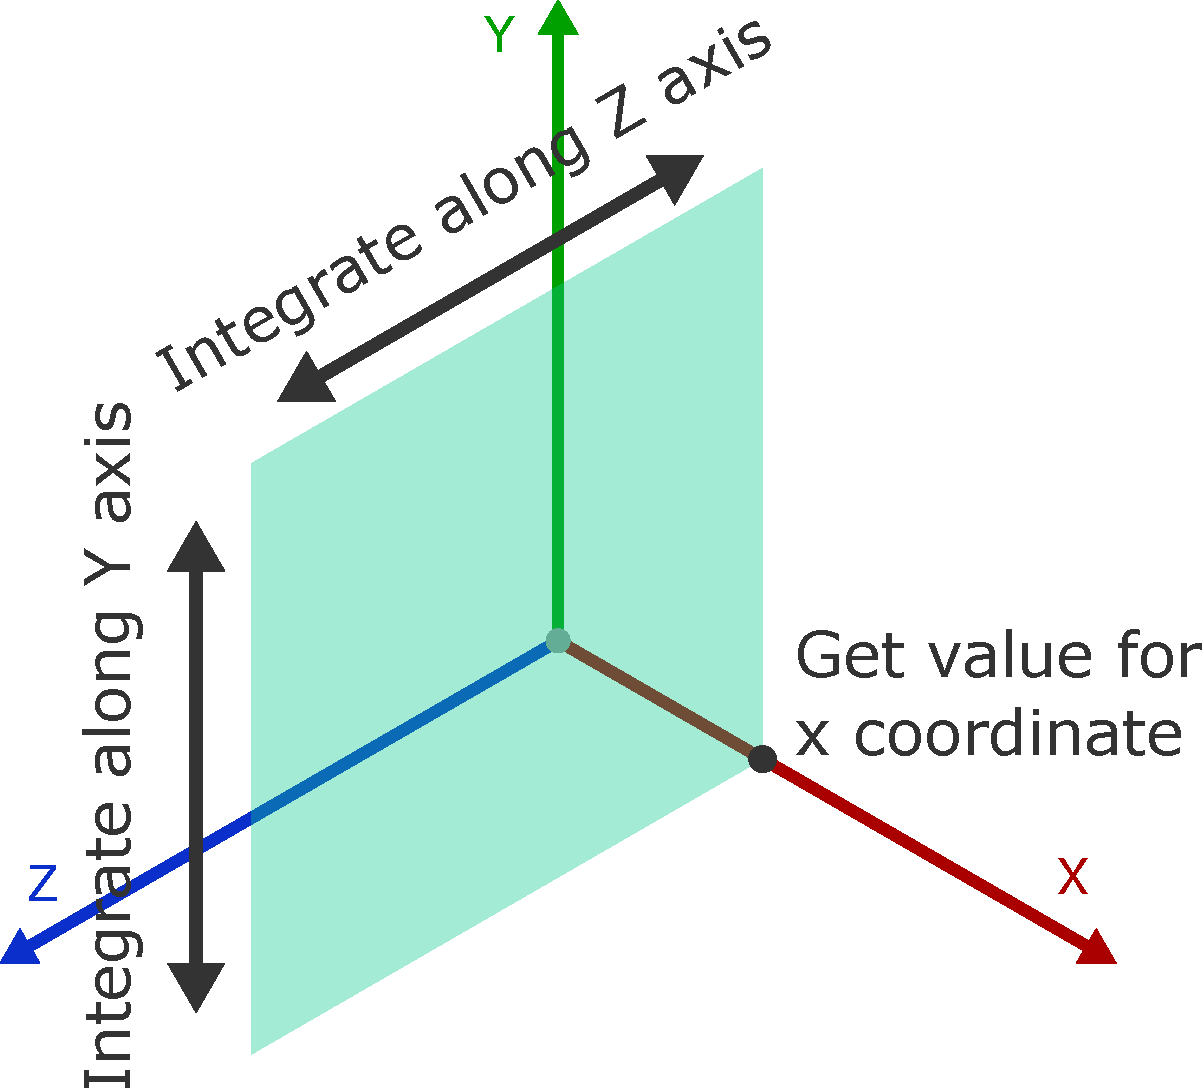
\includegraphics[width=0.5\textwidth]{figures/per_axis_plot_explained.pdf}
	\caption{Calculation method of the \textit{Per axis probability density} for a given $x$ coordinate}
	\label{fig:per_axis_explained}
\end{figure}
To obtain the plot of $\rho_X(x, t)$ per axis probability density, we integrate the $\rho(\vec{r}, t)$ where $r_x = x$ and the other two coordinates run across their domain.
Equation \ref{eq:per_axis_calculation} gives the formula for calculating this measurable for the $X$ axis.
\begin{equation}
	\rho_X(x, t) = \int_Y \int_Z \rho(\vec{r}, t)\; dy dz
	\label{eq:per_axis_calculation}
\end{equation}
Figure \ref{fig:per_axis_explained} attempts to provide further intuition.
We also overlap the plot of the potential barriers on the same graph to understand the changes in the propagation of the wave packet caused by the localized potential.
This type of plot can provide helpful information for most simulation cases. It is beneficial when we want to simulate the behavior of three one-dimensional particles in a three-dimensional configuration space.
In this case, the projected probability density along each axis represents the wave packet of a different 1D particle.
It is possible to initialize a potential that models the collision between these three particles.
This creates the effect that the particles interact.
In the configuration file, there is a possibility to set whether a potential barrier should appear in the visualization.
By disabling the visualization of the interaction potential, we can get rid of any hardly conceptualizable elements of the resulting potential and maybe focus on a wall or a harmonic oscillator instead.
Probability density 3D is the most self-explanatory output of the system.
Here, we take the probability density as a 3D volumetric data set and visualize it using ray tracing.
Ray tracing is the method where we conceptually shoot rays of light from the virtual camera through the visualized volume.
Figure \ref{fig:ray_tracing_method} explains the concept of ray tracing.
\begin{figure}
	\centering
	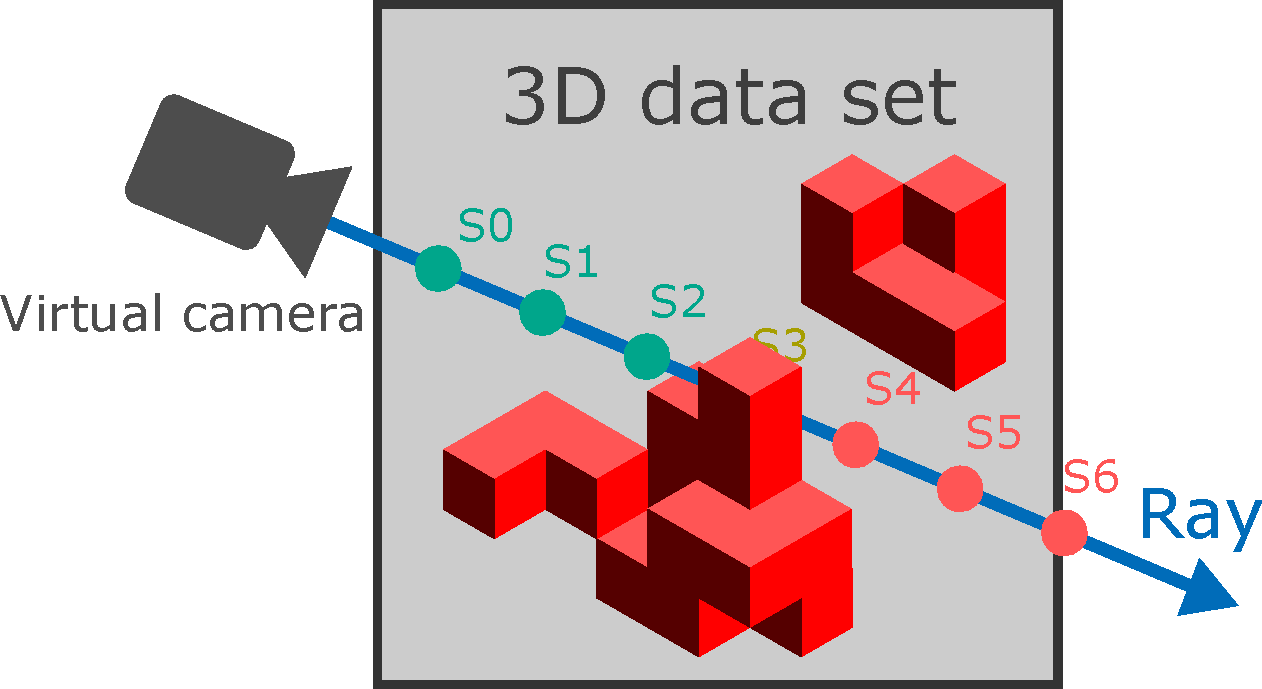
\includegraphics[width=0.75\textwidth]{figures/ray_tracing_visualization.pdf}
	\caption{Visual explanation of the ray tracing method: we sample the 3D data set along rays shot from the virtual camera}
	\label{fig:ray_tracing_method}
\end{figure}
For each pixel of the image, there is exactly one ray.
We progress along the ray in discrete steps, and at each step, we sample the data set.
The data read from the volume usually has a single intensity value.
We interpret the data using a transfer function that determines the color and opacity that should be associated with the intensity.
The color and opacity are then combined along the ray, resulting in the final color and opacity value for the image's pixel.
The operator that recursively combines the color and opacity values is called under operator. For recursive calculation of the $A_n$ opacity in $n$th step along the ray, it can be written in the form of
\begin{equation}
	\label{eq:under_op}
	A_n = A_{n-1} + \alpha_n(1 - A_{n-1})
\end{equation}
where $A_{n-1}$ is the opacity calculated at the previous step and $\alpha_n$ is the local opacity at the $n$th step.
A similar equation could be written for red, green, and blue (RGB) color channels.
If we would only use the colors obtained by simply stepping through the sample points, the look of the probability density would be rather dull.
We also utilize approximated gradient vectors.
One can calculate these vectors by taking the central difference using six additional samples around the currently sampled point.
(We, however, deployed a better method described later.)
The gradient vector points towards the direction in which the probability density increases the fastest.
If we make the analogy that a solid body object also has gradient vectors right on the edge of its surface so that these vectors point towards the inside of the object perpendicular to the surface,
we can make the connection between gradient vectors and surface normals.
Normal vectors of a surface are unit-length vectors pointing towards the outside world from the surface and are also perpendicular to the surface.
Normal vectors can be expressed as negated and normalized gradients.
Normal vectors are often used in various surface shading models since they give a good description of how surfaces reflect light.
Even though our probability density has a much less clearly defined gradient, this technique can still be used to obtain an approximated normal vector.
If this vector is sufficiently defined (the magnitude of the gradient is not too close to zero), then we can use a simple shading model such as the Blinn-Phong reflection model \cite{Blinn1977} to enhance our visuals.
We even use the length information of the gradient to fade between the shaded and unshaded look.
We would like to mention that in our previous works, we have experimented with more physically plausible shading techniques, such as applying the Cook-Torrance \acrfull{brdf} \cite{CookTorrance1982}.
This, however, has not yielded good results for volumetric visualization since surface imperfections are calculated into the model; thus, the generally fussy nature of volumetric data sets results in an overall dark look.
The simple Blinn-Phong model, however, is cheap to compute and provides sufficiently strong specular highlights while it's still easy to parameterize.
For most of our simulations, we use a total simulated volume of $512\times 512 \times 512$ data points.
We leave the outer half of the total volume to accommodate the draining potential described in the last part of section \ref{sec:used_method}.
This means that so far, we only visualize $50\%$ of the stored data set: $256 \times 256 \times 256$.
In the future, we may experiment with reducing the space used up by the draining potential.
Until then, we rely heavily on good reconstruction filters to get rid of the aliasing effects visible by sampling the data set of relatively low resolution.
We utilize Balázs Csébfalvi's reconstruction filter \cite{csebfalvi2023}.
This method provides consistent gradient estimation, that is, the analytic gradient of the reconstructed function.
It has an approximation order of three, and it is also $C^1$ continuous.
This method evaluates eight trilinear samples to calculate the intensity and the gradient for a given point.
In the current generation of \acrshort{gpu}s trilinear filtering can be efficiently evaluated using the built-in sampling routines.
The eight is only one more sample compared to the seven used in the less advanced intensity plus central difference technique, and we also get better results, as shown in the referred paper.

The last type of the five different image outputs of our program we call \textit{Probability evolution}.
To create this output, we divided the visible region of the simulated volume into separate partitions.
On these images of this type, we display a plot where we integrate the probability density over these regions following equation \ref{eq:probability_evolution}.
\begin{equation}
	\probP(t)=\int_\mathcal{V}\rho(\vec{r},t)d^3r
	\label{eq:probability_evolution}
\end{equation}
Conceptually, this gives us the probability of the event of the particle being found in these spatial regions.
It is also allowed to specify overlapping regions.
By doing so, we only get the probability of non-excluding events.
We prefer to create a measurement region for the entirety of the visible volume.
This is very informative when the particle leaves the visible parts. Hence, the probability of the particle being found somewhere inside the visible part drops below one.
Note that modeling such scenarios is made possible by using the draining potential.

Besides the sequence of images, our program also renders two animations in MP4 format.
One is created from a sequence of images rendered as in the \textit{Probability density 3D} sequence.
The other is the animated version of the \textit{Per axis probability density} sequence.
The rate at which the state of the simulation is captured as an animation frame and the playback frame rate can be configured separately.

\subsection{Performance test}

We measured the performance of our application.
We used a personal laptop to run and test the program.
The system specification of our computer is summarized in figure \ref{fig:system_spec}.
\begin{figure}
	\begin{center}
		\begin{tabular}{|m{5em}||m{25em}|}
			\hline
			CPU & AMD Ryzen 5 6600H with Radeon Graphics            3.30 GHz\\
			\hline
			GPU & NVIDIA GeForce RTX 3050 Ti Laptop GPU\\		
			\hline
			RAM & 16 GB\\		
			\hline
			OS & MS Windows 11 64-bit\\		
			\hline
		\end{tabular}
		\caption{System specification of the used test hardware}
		\label{fig:system_spec}
	\end{center}
\end{figure}
First, we tried a \acrshort{cpu}-only version of our simulator to compare the results with the \acrshort{gpu} accelerated implementation.
The results of the comparison can be found in figure \ref{fig:performance_test}.
\begin{figure}
	\begin{center}
		\begin{tabular}{|m{8em}||m{8em}| m{8em}| m{4em}|}
			\hline
			Input size & CPU-only Avg. [iter/s] & GPU~accelerated Avg. [iter/s] & Avg. speed up\\
			\hline
			$128 \times 128 \times 128$ & $1.1$ & $11.5$ & $\times 10.45$\\
			\hline
			$256 \times 256 \times 256$ & $0.09$ & $6.5$ & $\times 72.22$\\
			\hline
			$512 \times 512 \times 512$ & $0.01$ & $0.5$ & $\times 50.00$\\
			\hline
		\end{tabular}
		\caption{Results of a performance test using a CPU-only and a \acrshort{gpu} accelerated version of the application averaged}
		\label{fig:performance_test}
	\end{center}
\end{figure}
Here, we tested three different configurations with varying resolutions.
We measured the average iteration count per second.
The test shows that by using \acrshort{gpu} acceleration, we obtained significant speed up over the \acrshort{cpu}-only implementation.






